\documentclass[11pt]{article}
\usepackage{amsmath, amssymb}
\usepackage{graphicx}

\title{CS474 HW5}
\author{Evan Litzer}
\date{4/25/26}

\begin{document}

\maketitle

\section*{1A}

Data points are $(-1, -1)$, $(0, 0)$, $(1, 1)$

\[
\frac{-1 + 0 + 1}{3} = 0
\]

\[
\frac{-1 + 0 + 1}{3} = 0
\]

So mean $\mu = (0, 0)$ which means all of the data is centered.

All points lie on the line $y = x$

So all of the variation is in the direction of $(1, 1)$ and none is in direction of $(1, -1)$

Direction vector = $(1, 1)$

Unit direction vector:

Vector length = $\sqrt{a^2 + b^2}$

So for $(1, 1)$

\[
\|(1, 1)\| = \sqrt{1^2 + 1^2} = \sqrt{2}
\]

Then,

\[
u_1 = \frac{(1, 1)}{\|(1, 1)\|} \rightarrow u_1 = \frac{(1, 1)}{\sqrt{2}} \rightarrow u_1 = \left(\frac{1}{\sqrt{2}}, \frac{1}{\sqrt{2}}\right)
\]

Therefore, principal component is:

\[
u_1 = \left(\frac{1}{\sqrt{2}}, \frac{1}{\sqrt{2}}\right)
\]

Every point lies on the $y = x$ line and projecting onto the line will maintain all of the variation as there is no other direction to project in. The direction of maximum variance is line $y = x$, so first principal component is the unit vector along that line.

\section*{1B}

Principal component $u_1 = \left(\frac{1}{\sqrt{2}}, \frac{1}{\sqrt{2}}\right)$

Original coordinates $(-1, -1)$, $(0, 0)$, $(1, 1)$

PCA to one dimension will convert every point to having one coordinate instead of two. The one coordinate is how far it is along the direction of the PC

Therefore the 1D value for each point is the projection onto $u_1$

Data is centered so do not need to subtract mean $(x - \mu)$

\[
z = x^T u_1
\]

Plug in PC to get:

\[
z = x_1 \left(\frac{1}{\sqrt{2}}\right) + x_2 \left(\frac{1}{\sqrt{2}}\right)
\]

$(-1, -1)$ Point:

\[
z = (-1)\left(\frac{1}{\sqrt{2}}\right) + (-1)\left(\frac{1}{\sqrt{2}}\right)
\]

\[
= -\frac{1}{\sqrt{2}} - \frac{1}{\sqrt{2}} = -\frac{2}{\sqrt{2}} = -\sqrt{2}
\]

$(0, 0)$ Point:

\[
z = (0)\left(\frac{1}{\sqrt{2}}\right) + (0)\left(\frac{1}{\sqrt{2}}\right)
\]

\[
= 0 + 0 = 0
\]

$(1, 1)$ Point:

\[
z = (1)\left(\frac{1}{\sqrt{2}}\right) + (1)\left(\frac{1}{\sqrt{2}}\right)
\]

\[
= \frac{1}{\sqrt{2}} + \frac{1}{\sqrt{2}} = \frac{2}{\sqrt{2}} = \sqrt{2}
\]

Combining the three above results then becomes the 1D data $-\sqrt{2}, 0, \sqrt{2}$ and the 1D vectors are:

\[
[-\sqrt{2}], [0], [\sqrt{2}]
\]

\section*{2}

\begin{tabular}{c|ccccc}
 & p1 & p2 & p3 & p4 & p5 \\
\hline
p1 & 1.00 & 0.10 & 0.41 & 0.55 & 0.35 \\
p2 & 0.10 & 1.00 & 0.64 & 0.47 & 0.98 \\
p3 & 0.41 & 0.64 & 1.00 & 0.44 & 0.85 \\
p4 & 0.55 & 0.47 & 0.44 & 1.00 & 0.76 \\
p5 & 0.35 & 0.98 & 0.85 & 0.76 & 1.00 \\
\end{tabular}

\subsection*{Single Link Hierarchical Clustering}

First merge $p2$ and $p5$ to $\{p2, p5\}$ because $p2$ and $p5$ have the maximum similarity of $0.98$

\[
\begin{array}{c|cccc}
 & p1 & p3 & p4 & \{p2,p5\} \\
\hline
p1 & 1.00 & 0.41 & 0.55 & 0.35 \\
p3 & 0.41 & 1.00 & 0.44 & 0.85 \\
p4 & 0.55 & 0.44 & 1.00 & 0.76 \\
\{p2,p5\} & 0.35 & 0.85 & 0.76 & 1.00 \\
\end{array}
\]

Then merge $\{p2, p5\}$ with $p3$ into $\{p2, p3, p5\}$ because $p3$ has the maximum similarity with $\{p2, p5\}$

\[
\begin{array}{c|ccc}
 & p1 & p4 & \{p2,p3,p5\} \\
\hline
p1 & 1.00 & 0.55 & 0.41 \\
p4 & 0.55 & 1.00 & 0.76 \\
\{p2,p3,p5\} & 0.41 & 0.76 & 1.00 \\
\end{array}
\]

Merge $\{p2,p3,p5\}$ with $p4$ since $0.76$ is the largest single link similarity remaining.

\[
\begin{array}{c|cc}
 & p1 & \{p2,p3,p4,p5\} \\
\hline
p1 & 1.00 & 0.55 \\
\{p2,p3,p4,p5\} & 0.55 & 1.00 \\
\end{array}
\]

Then the final merge is $p1$ joining the cluster with similarity $0.55$.

So the single link merge order and dendrogram heights are:

\[
\{p2, p5\} \text{ with } 0.98 \text{ similarity and distance } 0.02
\]

\[
\{(p2,p5),p3\} \text{ with } 0.85 \text{ similarity and distance } 0.15
\]

\[
\{(p2,p5),p3),p4\} \text{ with } 0.76 \text{ similarity and distance } 0.24
\]

\[
\{(p2,p5),p3),p4),p1\} \text{ with } 0.55 \text{ similarity and distance } 0.45
\]

But only need 3 clusters, so the 3 clusters are $\{p2,p3,p5\}, \{p4\}, \{p1\}$

\begin{figure}[h]
    \centering
    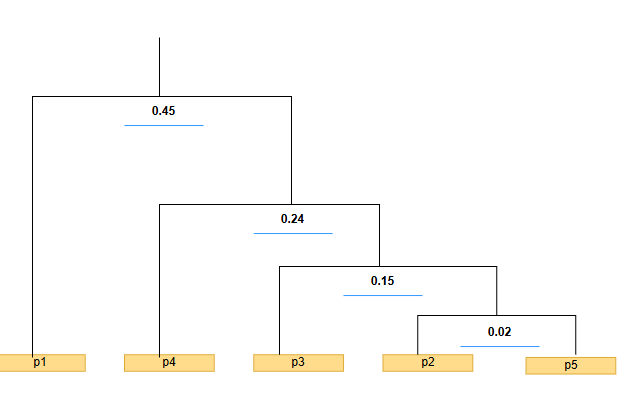
\includegraphics[width=0.8\textwidth]{single_link_dendrogram.png}
    \caption{Single Link Dendrogram}
\end{figure}

\subsection*{Complete Link Clustering}

Merge $p2$ and $p5$ because they have the largest similarity and are not clustered yet.

\[
\begin{array}{c|cccc}
 & p1 & p3 & p4 & \{p2,p5\} \\
\hline
p1 & 1.00 & 0.41 & 0.55 & 0.10 \\
p3 & 0.41 & 1.00 & 0.44 & 0.64 \\
p4 & 0.55 & 0.44 & 1.00 & 0.47 \\
\{p2,p5\} & 0.10 & 0.64 & 0.47 & 1.00 \\
\end{array}
\]

The biggest similarity is $s(\{p2,p5\},p3) = 0.64$

Merge $\{p2, p5\}$ with $p3 \rightarrow \{p2, p3, p5\}$

\[
\begin{array}{c|ccc}
 & p1 & p4 & \{p2,p3,p5\} \\
\hline
p1 & 1.00 & 0.55 & 0.10 \\
p4 & 0.55 & 1.00 & 0.44 \\
\{p2,p3,p5\} & 0.10 & 0.44 & 1.00 \\
\end{array}
\]

The biggest similarity is $s(p1,p4) = 0.55$

Merge $p1$ and $p4 \rightarrow \{p1,p4\}$

\[
\begin{array}{c|cc}
 & \{p1,p4\} & \{p2,p3,p5\} \\
\hline
\{p1,p4\} & 1.00 & 0.10 \\
\{p2,p3,p5\} & 0.10 & 1.00 \\
\end{array}
\]

Then the final merge is $\{p1, p4\}$ with $\{p2,p3,p5\}$ with similarity $0.10$.

So the dendrogram/order is:

\[
(p2,p5) \text{ with } 0.98 \text{ similarity and } 0.02 \text{ distance}
\]

\[
((p2,p5),p3) \text{ with } 0.64 \text{ similarity and } 0.36 \text{ distance}
\]

\[
(p1,p4) \text{ with } 0.55 \text{ similarity and } 0.45 \text{ distance}
\]

\[
((p2,p3,p5),(p1,p4)) \text{ with } 0.10 \text{ similarity and } 0.90 \text{ distance}
\]

Since it is only a 3 link cluster, then the 3 clusters are $\{p2,p3,p5\}, \{p1\}, \{p4\}$

\begin{figure}[h]
    \centering
    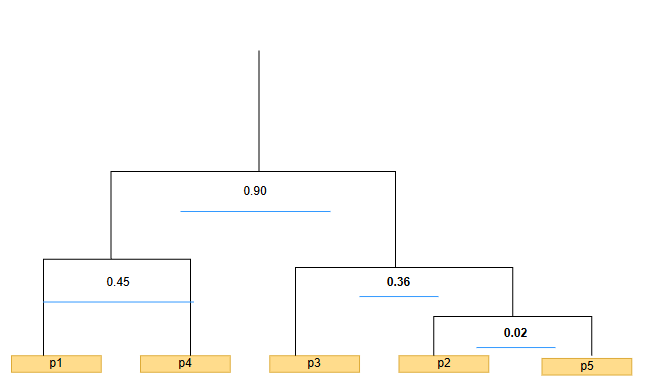
\includegraphics[width=0.8\textwidth]{complete_link_dendrogram.png}
    \caption{Complete Link Dendrogram}
\end{figure}

\section*{3A}

The input is $X \in \mathbb{R}^{64 \times 64 \times 128}$

Convolutions use padding $p = 1$ and $3 \times 3$ kernels.

Layer 1:

$3 \times 3$ kernel with stride $= 2$

Input $64 \times 64 \times 128$ and output

\[
\frac{64 + (2*1) - 3}{2} + 1 = 32
\]

So output is $32 \times 32 \times 256$

Parameters are

\[
3 * 3 * 128 * 256 = 294912
\]

Layer 2:

$3 \times 3$ kernel with stride $= 1$

Input is $32 \times 32 \times 256$ and output is

\[
\frac{32 + 2*1 - 3}{1} + 1 = 32
\]

So output is $32 \times 32 \times 512$

Parameters are

\[
3 * 3 * 256 * 512 = 1179648
\]

Total parameters

\[
= 294912 + 1179648 = 1474560
\]

\section*{3B}

Layer 1:

$3 \times 3$ kernel with stride $= 2$

Input $64 \times 64 \times 128$ and output

\[
\frac{64 + (2*1) - 3}{2} + 1 = 32
\]

So output is $32 \times 32 \times 256$

Multi-add operations:

\[
32 * 32 * 256 * 3 * 3 * 128 = 301989888
\]

Layer 2:

$3 \times 3$ kernel with stride $= 1$

Input is $32 \times 32 \times 256$ and output is

\[
\frac{32 + 2*1 - 3}{1} + 1 = 32
\]

So output is $32 \times 32 \times 512$

Multi add operations:

\[
32 * 32 * 512 * 3 * 3 * 256 = 1207959552
\]

Total multi add operations:

\[
301989888 + 1207959552 = 1509949440
\]

\section*{3C}

Layer 1:

$3 \times 3$ kernel with stride $= 2$

Input $64 \times 64 \times 128$ and output

\[
\frac{64 + (2*1) - 3}{2} + 1 = 32
\]

So output is $32 \times 32 \times 256$

Layer 2:

$3 \times 3$ kernel with stride $= 1$

Input is $32 \times 32 \times 256$ and output is

\[
\frac{32 + 2*1 - 3}{1} + 1 = 32
\]

So output is $32 \times 32 \times 512$

Input feature size:

\[
64 * 64 * 128 = 524288
\]

Output feature size:

\[
32 * 32 * 512 = 524288
\]

Change:

\[
\frac{524288 - 524288}{524288} * 100 = 0
\]

\[
0\% \text{ change}
\]


\end{document}